% !TeX spellcheck = en_US
\documentclass[11pt,a4paper]{article}
\usepackage[utf8]{inputenc}
\usepackage{amsmath}
\usepackage{amsfonts}
\usepackage{amssymb}
\usepackage{graphicx}
\usepackage{mathtools}
\usepackage[hidelinks]{hyperref}  % most people dont know of this :3

\usepackage{booktabs}
\usepackage{tabularx}

\usepackage{subfig}
% \usepackage[margin=0.7in]{geometry}

\usepackage[backend=bibtex,style=verbose-ibid]{biblatex}
\addbibresource{citations.bib}

\usepackage{listings}
\usepackage{color}
\definecolor{dkgreen}{rgb}{0,0.6,0}
\definecolor{gray}{rgb}{0.5,0.5,0.5}
\definecolor{mauve}{rgb}{0.58,0,0.82}

\lstset{frame=tb,
  language=Python,
  aboveskip=3mm,
  belowskip=3mm,
  showstringspaces=false,
  columns=flexible,
  basicstyle={\small\ttfamily},
  numbers=none,
  numberstyle=\tiny\color{gray},
  keywordstyle=\color{blue},
  commentstyle=\color{dkgreen},
  stringstyle=\color{mauve},
  breaklines=true,
  breakatwhitespace=true,
  tabsize=3
}

\providecommand{\main}{..} 
\graphicspath{{\main/images/}{images/}}


\author{jcn514}
\title{IB Music Exploring Portfolio}
\date{\today}

\begin{document}
\maketitle
\tableofcontents

\pagebreak

\iffalse
heres an example of a code block
\begin{lstlisting}
        def intervalValues(z, n):
            return output $\sharp$ return the sequence of values
\end{lstlisting}

heres an example of an image
\begin{figure}[h]
\begin{center}
\includegraphics[scale=.37]{onefifteen} 
\caption{Sequences Generated by n = 1-15 on Argand Diagram}
\end{center}
\end{figure}
\fi

\section{Introduction}
In my explorational journey, I frequently encounter new styles, genres, techniques and theory that challenge my assumptions about music. Across a number of AOIs, I find myself pouring through musical scores, in combination with listening, sight-reading, and analyzing, trying to grasp at a genre’s conventions or motifs. One particular genre that piqued my interest was videogame music. To me, it’s fascinating how videogames leverage techniques from a deluge of genres, yet still conform to the technical or physical limitations of a game. For instance, a number of songs I analyzed utilize only the square, sawtooth, and triangle tones due to the limitations of the original NES, making complex instrumentation or intricate polyphony impossible. Despite this, video game composers manufacture memorable, impactful music that often stands alone as a work of art, irrespective of the game it's in. This provoked me to explore how this type of music could act as both music for listening (AOI 2) and music to complement a game or other medium (AOI 3). I researched the intergenre connections among videogames music, classical impressionism and early ragtime/jazz, discovering surprising connections. To experiment with these fascinating ideas, this led me to perform a cover of a videogame classic in the style of ragtime and to create an arrangement of an orchestral videogame song for piano duet, falling under AOI 2 and 3 respectively.

\section{Research}

\subsection{Research 1: Country Club Rag}

In focusing on AOI 2, I explored ragtime piano. To understand the key characteristics/tropes of the genre, I explored the music of many staple composers in the transition from ragtime to its successor, jazz, including James P. Johnson, and Ubie Blake. I focused on Scott Joplin’s work, of which "Maple Leaf Rag" and "The Entertainer" are the most well-known. Within the historical context of the American South, his rise to prominence reflects perseverance within the African-American community, as well as the innovative applications of African rythems to 'western' (loosely-speaking) instruments.
His “Country Club Rag” is an insightful case study on his style. The composition is in a repetitive arrangement form: AABBCCDD. Patterning the genre, the piece has a playful and energetic tone, highlighted by bouncing rhythms and driven harmony. The first four introductory bars establish a motif of chromaticism until culminating with a V-I cadence to the tonic, both of which emblematic of the genre's style. From here, the piece utilizes a syncopated LH motif. Informed by the ‘march’ style and traditional African polyrhythms, the pattern of bass notes on the strong beats (1-3) and chords on the weak beats (2-4).  The song remains in its key-center, besides the secondary dominants and borrowed chords throughout—hinting at jazz. 
\begin{figure}[ht]
\begin{center}
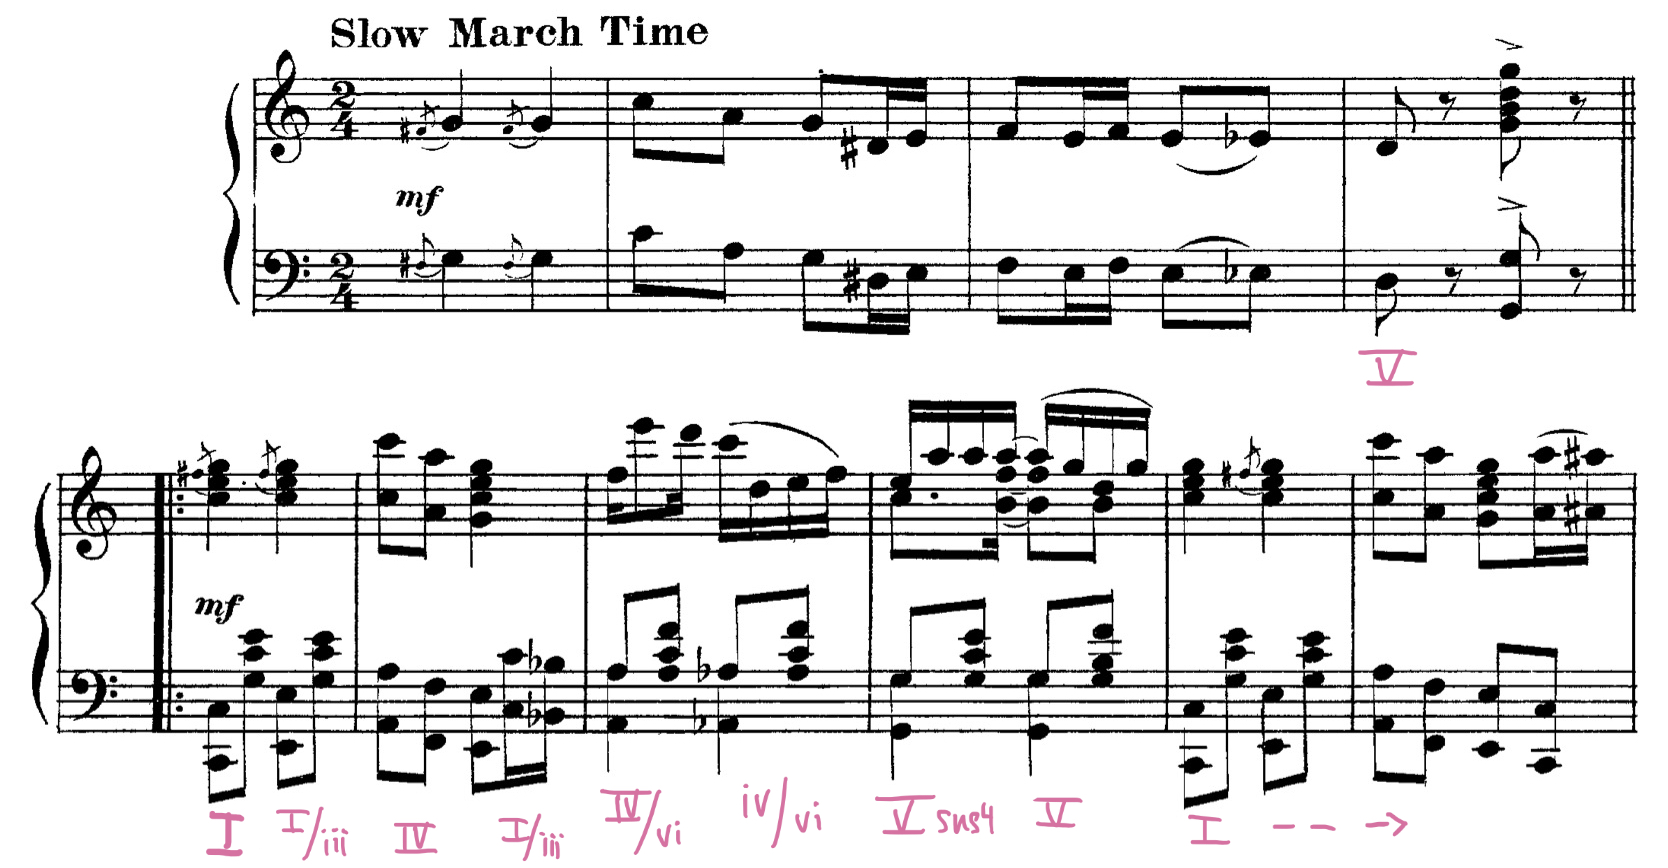
\includegraphics[width=\linewidth]{country} \\
\caption{Measures 1-10 of Joplin's "Country Club Rag" (public domain)}
\label{fig:joplin}
\end{center}
\end{figure}
For instance, measures 11–13 have an unconventional VII7-iii-V7-I cadence, wherein a iii-V\footnote{In the major key, iii can be considered dominant-parallel, which I am assuming here} movement is preceded by Em's secondary dominant, B7. Another important element of this piece is the use of the II7 chord, functioning as a secondary dominant (or as a passing diminished when the II7’s root note is omitted) into the dominant V chord of the home key. In this way, the piece encourages the listener to firmly grasp the direction of the harmony—each note resolves in a predictable, directional manner. The entire piece has a texture consisting of two distinct layers: the bottom bass rhythm and the chromatic melody on top. Overall, these elements are archetypal to the ragtime genre and pinpoint Joplin’s unique stylistic conventions. Despite the similarities to other songs in the ragtime genre, country club rag stands out as possibly more harmonically engaging than most. This is because Country Club Rag features certain elements of early jazz music, such as a walking baseline and borrowed chords. This combined with heavy chromaticism gives Country Club Rag a unique vibe compared to more stereotypical Joplin works like The Entertainer.\autocite{joplin}


\subsection{Research 2: Piano Concerto for the Left Hand}

Ravel’s Piano Concerto for the Left Hand stands as one of his most unique works. As one of his post-WWI works, it displays a marked shift in his style, mirroring the aftermath of France after the war. To study the art of this time period, I also explored works by Ravel's contemporaries, including Claude Debussy, Eric Satie, and Honneger among others. This piece was commissioned by Paul Wittgenstien, an Austrian pianist who lost his right arm as a soldier.\autocite[100]{Orenstein} This concerto is fascinating both in its technical accomplishment, but also in its marked jazz influence. Ravel composed this (and his G major concerto) after a multi-year-long trip to the United States, where he was introduced to the beginnings of jazz. In a public lecture on contemporary music, Ravel was quoted, “[M]ay this national American music of yours embody a great deal of the rich and diverting rhythm of your jazz, [...] worthily deriving from, and in turn contributing to, a noble heritage in music” (Arbie 98). The culmination of these factors is a concerto that is remarkable for its orchestration, its avant-garde, its technical challenge, and, above all, its spirit.
 To glimpse at the genius of the entire piece, consider an analysis of the opening buildup to the piano cadenza: Ravel’s left-hand concerto introduces the first main melody in the lower register of a Contrabassoon overtop a muddy Em(add 4) harmony, before it moves down to rest on a C, outlining a C/E, which is then reinforced by the Bb in the Cornets giving it a mixolydian sound. Here, Ravel emphasizes this harmony as a Eø7 so as to prepare for the resolution to a D5 in the key of Dm. In a twist of expectations, he takes this fifth, voiced in the horns, a semitone down, establishing a new tonal center of C$\sharp$. This, with the transposed melody outlining a C$\sharp$m(maj 7)—harmonic minor harmony, ambiguously shifts to the III chord, E major. The melody in C$\sharp$ harmonic minor emphasizes the G$\sharp$, A$\sharp$, B$\sharp$—the 5th $\natural$6th and $\natural$7th scale degrees respectively—which then changes subtly changes to G$\sharp$, A$\sharp$, B$\natural$, outlining the $\natural$3rd, $\sharp$4th and 5th of the new harmony in E. Combined with the inclusion of the pulsing b7th in the strings, Ravel implies a challenging E-lydian-mixolydian mode (viz. A raised 4th and flattened 7th)—only one note from a whole-tone scale. As tension builds with a rising melody, this E serves as the dominant chord in a V-I resolution to A major. Quick to prevent this from sounding ‘resolved,’ Ravel incorporates the b7th in a rhythmic motif in the strings along with the b9th (The Bb an octave above the A) to outline a dominant b9 chord with a thick, oppressive texture in the orchestra. He grows and thickens this harmony incorporating a new counter-melody in the trumpets almost giving it a Dm/A or iv/i sound. This grows to an apex with a fortissimo Asus4 with a dominant function. Without resolving the dominant harmony, the piano cadenza begins with the same tonal center of A.\autocite{ravel}

\subsection{Research 3: Rudebuster}

For AOI 3, I chose to analyze ‘Rudebuster’ written by Toby Fox for the videogame Deltarune. Studying the genre of videogame music more broadly, I explored works from other influential japanese composers like Koji Kondo and Nobuo Uematsu; as well as American composes like Martin O'Donnell and Jeremy Soule. As it's primarily a backing track to another form of media, it's fascinating to explore how Fox contributes to the lively atmosphere using music. To complete this analysis, I also transcribed a reduction of the main harmony/ostinato.
In this piece, Toby Fox uses the phrygian mode and a syncopated rhythm to create an upbeat sound. The start clearly outlines the main progression of i-bII-bVI-V7 with an electronic piano-like sound. Notably, this chord progression takes place in a microtonal key just flat of G (G half-flat/F half-sharp), which I will hereafter spell as G. Percussion-wise, Fox makes use of an electronic drum set and noise synths/hi-hats. His snare and bass establish a backbeat anticipating beat 3, with a noise synth constant filling the empty space with the 16th notes. To produce the upbeat syncopation, the piano harmony, mirroring the drums, anticipates beat 3 and emphasizes the remaining weak beats. This piano ostinato is important in that it outlines chord extensions of the bass. For example, the piano begins with a Bb triad overtop a G in the bass implying a Gm7 harmony.
One notable feature of the song is its use of the phrygian b2 mode. In particular, the im7 to II6 movement gives the song a spicy twist, adding a jazzy feel that accentuates the syncopation. The remaining harmony reinforces the phrygian mode, with a typical v-i cadence mode-mixing the minor v chord from the tonic G’s typical minor/aeolian mode. Fox emphasizes this cross relation between the Db and D$\natural$, in his melody as well, highlighting the intention behind this choice.\autocite{rudebuster}

\subsection{Research 4: Wii Shop Channel Main Theme}

For this analysis, I chose the “Wii Shop Channel Main Theme.” This song, notorious for its catchy, bossa nova vibe, plays on Nintendo’s original Wii (game console) in the Shop app. This is AOI3 because its purpose is to act as background music as the user scrolls through menus and purchases games---much like the function of elevator music, etc.
    The song begins by establishing the key with a clear V13 dominant chord struck twice in the melody’s main synth. The percussion fills in the two measures following, outlining its notorious bossa nova rhythm. This style, translating literally to “new trend” or “new wave,” derives from the Brazilian samba and is known for its introduction of innovative syncopation to traditional samba rhythms. In a similar fashion, Wii Shop’s composers broke the traditional confines of video game music---which has a reputation for its electronic sound---instead combining a unique blend of live instruments, bass guitar, maracas, and wood blocks in addition to a single, unchanging synth.
    The Wii Shop theme is notable for its complex harmonies and jazz influence. Taking advantage of many chord extensions, its composers thoughtfully create harmonic variety despite its perceived simplicity. Another motif of its is the tendency to use ii-V-I turnarounds to either modulate or generate momentum within a key. For instance, shortly after establishing the main theme, the introduction modulates to an entirely new key through a ii-V-I turnaround. Its composers, wary of the need to avoid too much atonality, ground the listener through these modulations in its use of a ostinato 5--1 bassline in the bass guitar corresponding to the respective harmony. Despite the occasional voice-leading chromaticism, this baseline serves to reinforce where the listener is in the piece, making the numerous cross-relations, accidentals, modulations, etc more palatable.\autocite{wiishop}
    
\section{Exploring as a Performer Written Statement}

To explore unfamiliar territory as an arranger, I chose to reinvent an orchestral piece for four hands piano. My stimulus was “Main Theme” from Octopath Traveler, composed by Yasonuri Nishiki. I came across this song within a videogame I had not played. I was intrigued by the instrumentation and western style despite its Japanese origin. I hadn’t written for four hands on the piano; I was excited to undertake the challenge. Therefore, this project falls under Global Context and AOI 3, since I adapted music to an unfamiliar instrumentation and the music evokes emotion within the game. 

My initial brainstorm consisted of exploring unfamiliar music in a variety of genres. I decided on this arrangement after listening to the four-hands piano work of Schubert and Brahms, notably Schubert’s Sonata in C major for piano four-hands, D 812, wherein he utilizes block chords and intertwines melody between the primo and secondo players. I sought more research material to understand the facets of disseminating complex melodies and harmonies from many instruments to four hands. One tip I found helpful was not limiting my top voice to the melody; at times I had a pianissimo sans acentuacion ostinato in the top voice adding glitter to the harmony. Additionally, I incorporated a call/response melody in the treble of the secondo piano. Overall, I found my research into the conventions of four-hands piano useful in expanding my musical vocabulary within this style.

My 32-bar composition was the first section of the orchestral piece. Using piano dynamics, I tried to emulate the chugging chords in the strings section. In the first section, I also used acciaccatura to emulate the sound of wind instruments. I often deviated from the stimulus piece by adding in extra chord extensions and voicing the melody in 3rds 5ths and 6ths. After the sudden key change, I employed dynamic contrast between the secondo piano playing melody and the primo piano contributing to harmony with ostinato ‘trill-like’ chords using various diatonic 2nds in the appropriate mode (e.g., Ab lydian, Eb dorian, etc.). I included this novel motif throughout the piece because it added a ‘glitter-like’ feeling to the harmony. Lastly, I incorporated syncopation and thick cluster-chords to give the final two sections momentum and emphasis.

Overall, I was pleased with the outcome of my exploration, although it was more difficult than anticipated. Throughout the project, the most time-consuming part was adapting parts such that the pianists could play notes comfortably without overlapping. This had the effect of forcing me to interchange my melodies between hands and to write in some confusing fingerings. Despite the difficulty, I feel that I learnt a lot about composing for four hands piano during this process. If I were to complete this assignment once more, I would record each part since the sampled piano on the notation software made certain parts sound too muddy. By recording it, I would achieve more realistic dynamics between the melody and the filler notes within the chords.


\section{Exploring as a Creator Written Statement}

For the task of Exploring as a Performer, I chose the “World Ending Theme” from Super Mario World. This song falls under local context and the AOI 2: music for listening and performing. My relationship to this song prior to the project was limited, as I have never played Super Mario world. Yet, this has a local context because I enjoy listening to video game music in general. Furthermore, this piece falls into AOI 2 because I adapted this song to a rag-time genre, which is traditionally a performance-based convention. 
My initial brainstorming ideas included emphasizing the rag-time-like sound with a ‘jumping’ left-hand figure and an accentuation of the swing rhythm. I focused on maintaining the general structure and ‘feel’ of the harmony throughout; the major changes I made were in voicing chord extensions and voice-leading With these core ideas in mind, I set out to research rag-time conventions with which I had no experience. One interesting thing I encountered was the influence of Black Americans on popularising rag-time, especially in the realm of American pop music. One composer I focused primarily on was Scott Joplin. After listening to his style, I felt I had a strong foundation. Some techniques I tried to implement were the emphasis on the bass note on beats 1 and 3 with the chords played typically higher on beats 2 and 4, and the syncopated ‘swing’ melody. Some less prevalent conventions that provided a ‘ragtime-like’ feel were the interplay between the b3rd and 3rd note diatonically and the use of altered dominant chords.
 
For the first week, it was helpful to explicitly write out the melody so I could understand the swing rhythm. After this, the main portion of my adaptation was practicing the muscle memory for the jumps in the left-hand. Despite my experience with piano, I had not encountered many sections that had large jumps throughout. This also took time because I intentionally challenged myself with the intervals and the spacing. Using advanced conventions, I voiced the bass notes on beats 1 \& 3 using octaves and the chords on beats 2 \& 4 with a mix of inverted three and four-note chords. For these reasons, it was initially difficult to play both the RH and LH together. Another idea I developed during this time was tightening the voice leading by altering the chord extensions. One example of this was the ending 2-5-1 cadence that I spiced up by playing playing an Fmaj7 over D (Dm9), a F A$\sharp$ B Eb over G (Galt), and resolving to a Cmaj(6/9). Here for instance, the upper voice walks down two semitones from E to Eb to D throughout this cadence. In the original song, there is a frequent use of the ‘mario chord:’ an augmented dominant chord. I also worked extensively to include this within my arrangement and to use the augmented 5th in my voice leading.
 
As I progressed, the song became much easier and more enjoyable to play. Recording the performance was not terribly difficult; it only took around five takes. It also took a slight amount of work to set up the stereo microphone setup and to tweak my adjustments to the sound. Overall, from this assessment I have learned that my piano abilities are able to adapt to novel styles and situations, since I was able to perform in ragtime despite my inexperience. I really enjoyed exploring past the realms of classical music, wherein I have focused primarily on techniques like arpeggios and finger dexterity.

\section{Audio excerpts}

\begin{table}[ht]
\centering
\begin{tabularx}{0.9\textwidth}{@{}lX@{}}
\toprule
\textbf{Track}                                            & \textbf{Timestamp}                                                  \\ \midrule
Country Club Rag – Scott Joplin                  & 0:00                                                                \\[4pt]
Piano Concerto for the Left Hand – Maurice Ravel & \begin{tabular}[c]{@{}l@{}}PART 1: 0:41\\ PART 2: 1:05\end{tabular} \\[10pt]
Rude Buster – Toby Fox                           & 1:42                                                                \\[5pt]
Wii Shop Theme – Nintendo                        & 2:17                                                                \\ \bottomrule
\end{tabularx}
\caption{Audio tracks for Music Research}
\end{table}

\begin{table}[ht]
\centering
\begin{tabularx}{0.8\textwidth}{@{}lX@{}}
\toprule
\textbf{Track}                   & \textbf{Timestamp} \\ \midrule
Exploring as a Creator           & 0:00               \\
Ending Theme – Super Mario World & 1:13               \\
Exploring as a Performer         & 1:58               \\ \bottomrule     
\end{tabularx}
\caption{Audio evidence for Exploring as a Creator/Performer}
\end{table}


\pagebreak

\printbibliography

\end{document}